        	\begin{question}{1202}{Vecteurs}{1}{/}
				Soit un vecteur $\vec{A}=(a_x;a_y)$. Quelle est la norme de ce vecteur?
            \end{question}
            \begin{reponses}
            	\item[false] $a_x+a_y$
            	\item[false] $a_x\times a_y$
                \item[false] $a_{x}^2+a_{y}^2$
                \item[true] $\sqrt{a_{x}^2+a_{y}^2}$
            \end{reponses}
			%%%%%%%%%%%%%%%%%%%%%%%%%%%%%%%%%%%%%
        	\begin{question}{1202}{Vecteurs}{1}{/}
				Soit un vecteur $\vec{A}=(a_x;a_y;a_z)$. Quelle est la norme de ce vecteur?
            \end{question}
            \begin{reponses}
            	\item[false] $a_x+a_y+a_z$
            	\item[false] $a_x\times a_y\times a_z$
                \item[false] $a_{x}^2+a_{y}^2+a_{z}^2$
                \item[true] $\sqrt{a_{x}^2+a_{y}^2+a_{z}^2}$
            \end{reponses}
			%%%%%%%%%%%%%%%%%%%%%%%%%%%%%%%%%%%%%
            \begin{question}{1202}{Vecteurs}{2}{/}
                Quelle est la norme du vecteur $\vec{AB}$?
                \begin{center}
                	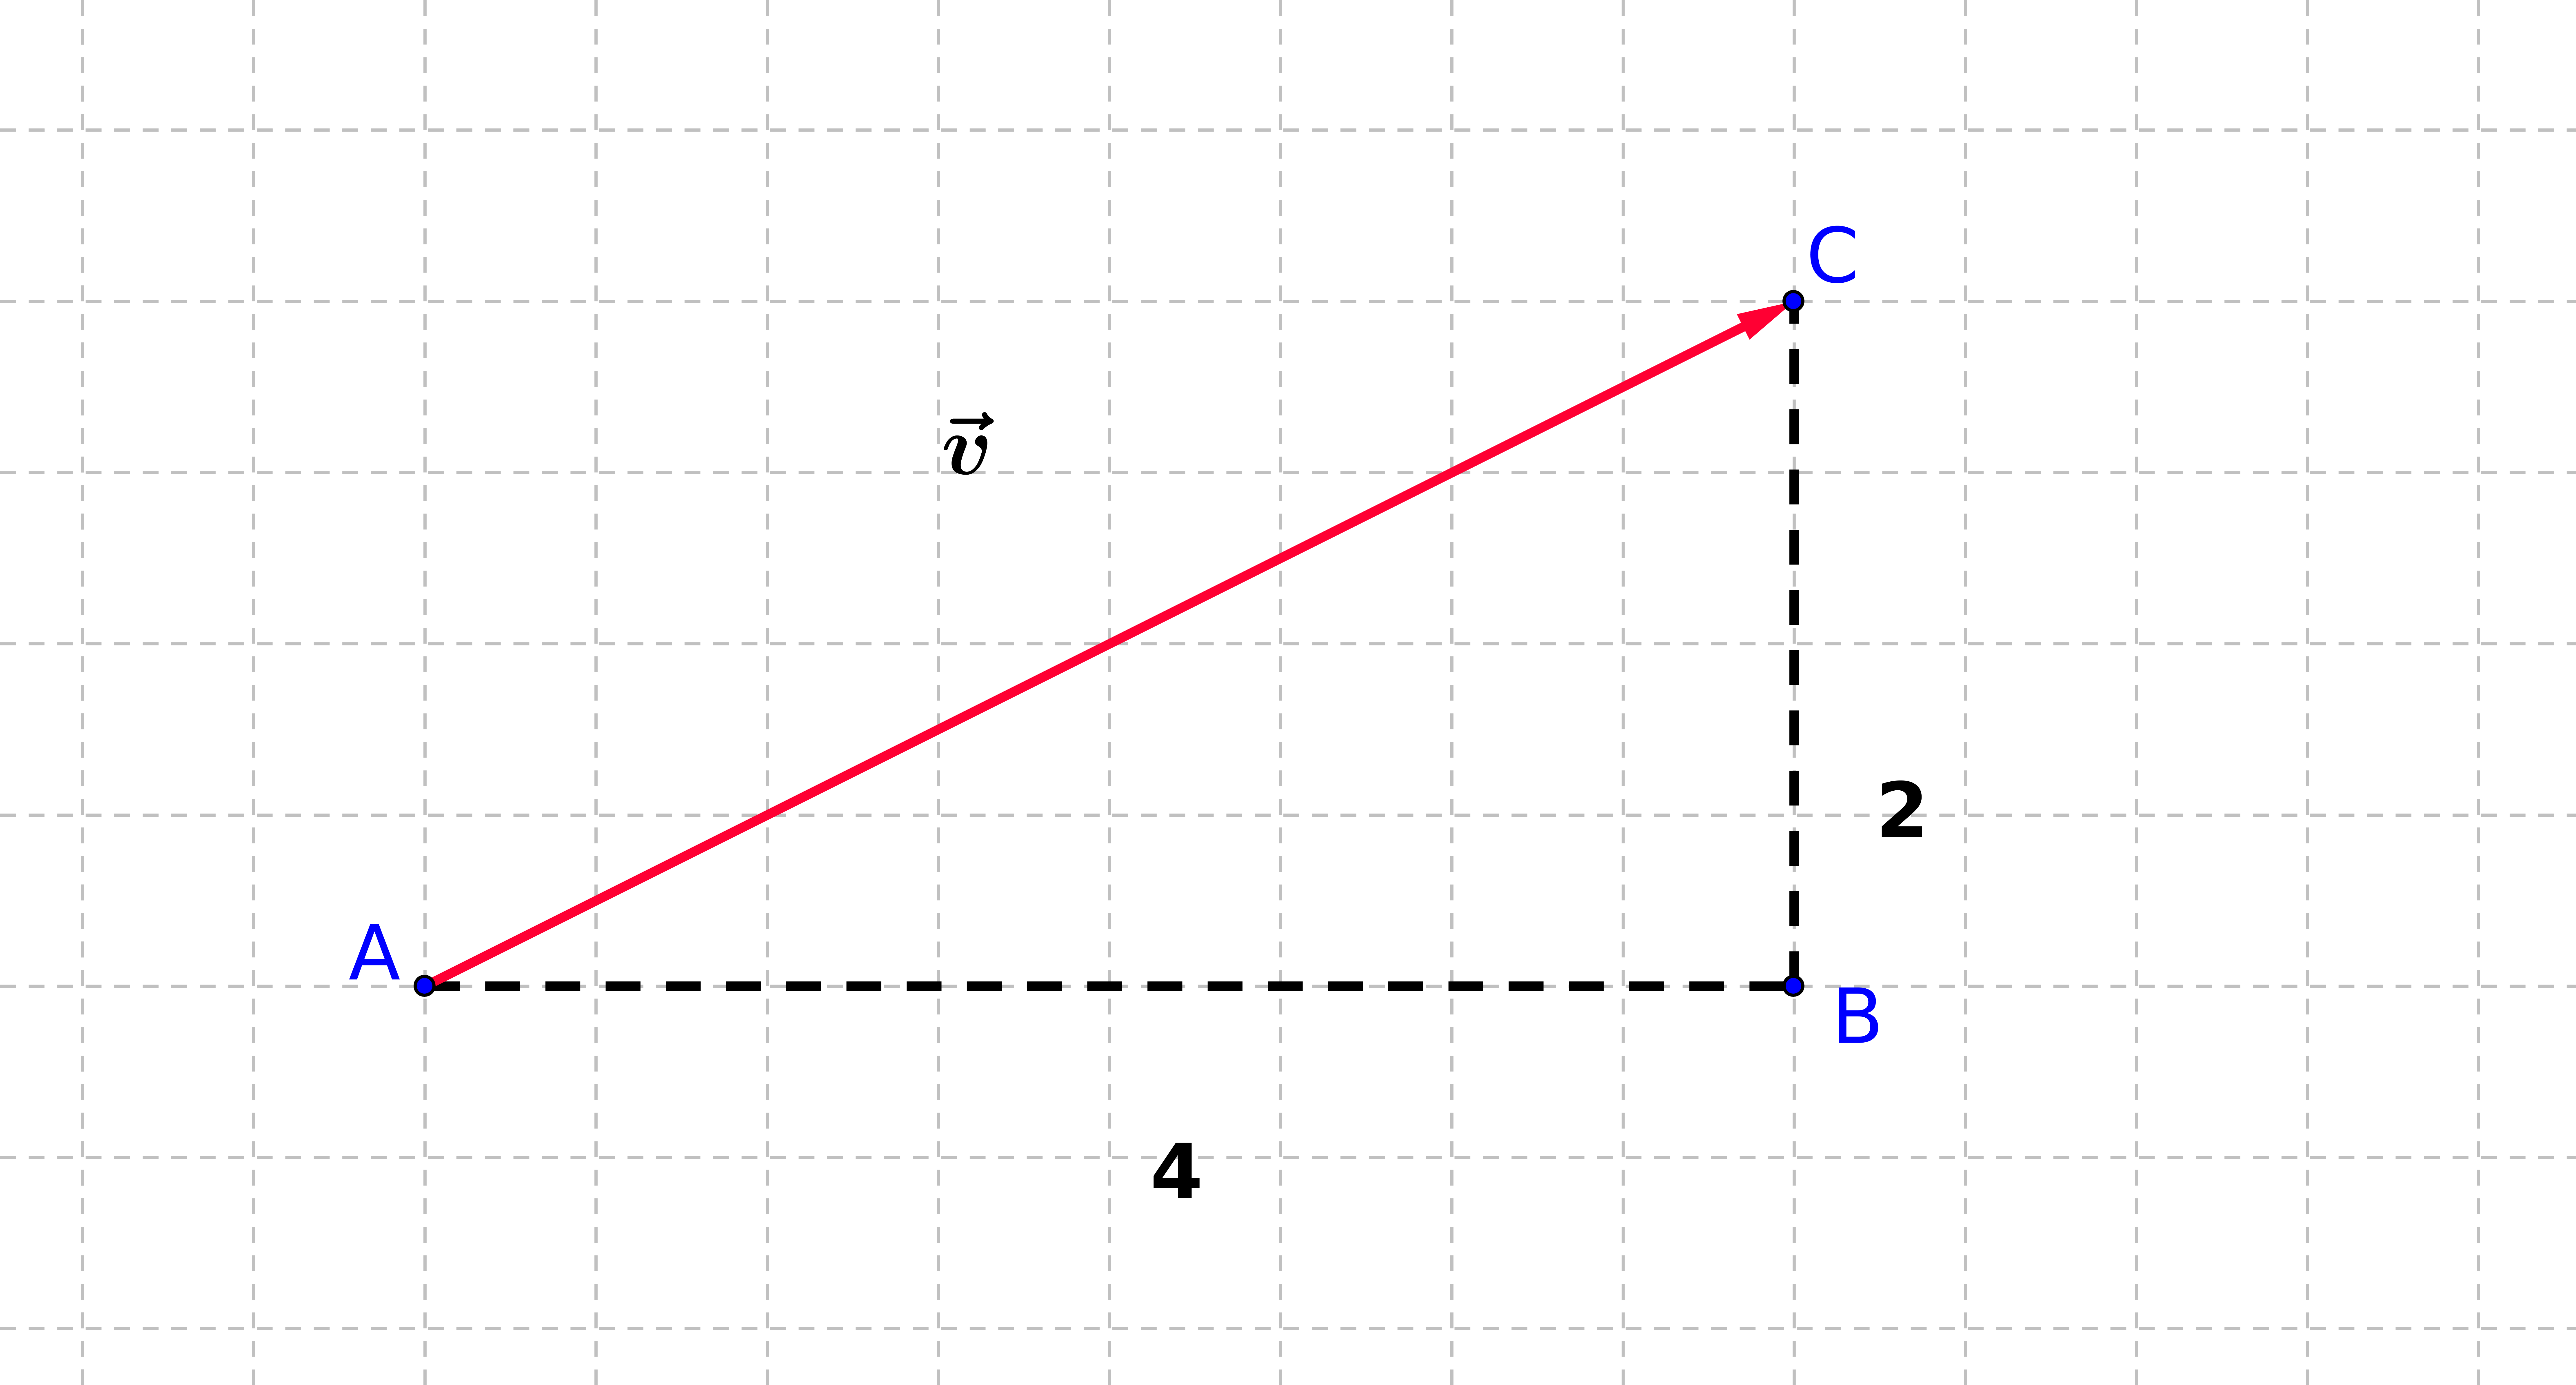
\includegraphics[width=0.5\textwidth]{Philippe/Figures_Philippe/vecteurs_4_2.png}
                \end{center}
            \end{question}
            \begin{reponses}
                \item[false] 6
                \item[false] $\sqrt{6}$
                \item[false] $20$
                \item[true] $\sqrt{20}$ 
            \end{reponses}
            %%%%%%%%%%%%%%%%%%%%%%%%%%%%%%%%%%%%%
            \begin{question}{1202}{Vecteurs}{2}{/}
                Un vecteur a pour coordonnées dans le plan: $x = 4$ et $y = 3$. Combien vaut sa norme?
            \end{question}
            \begin{reponses}
                \item[false] 6
                \item[true] 5
                \item[false] 7
                \item[false] 12
            \end{reponses}
            %%%%%%%%%%%%%%%%%%%%%%%%%%%%%%%%%%%%%
            \begin{question}{1202}{Vecteurs}{2}{/}
                Quelle est la norme $F$ du vecteur force de coordonnées dans le plan $\vec{F}=(12;5)$?
            \end{question}
            \begin{reponses}
                \item[true] \SI{13}{\newton}.
                \item[false] \SI{14}{\newton}.
                \item[false] \SI{15}{\newton}.
                \item[false] \SI{18}{\newton}.
            \end{reponses}
            %%%%%%%%%%%%%%%%%%%%%%%%%%%%%%%%%%%%%
